% !TEX TS-program = pdflatex
% !TEX root = ../tesi.tex

%************************************************
\chapter{My implementation}
\label{chp:fundamentals}
%************************************************

My main work is on audio implementation: i chose to use an open-source game written in C++ called "Cube".
Cube is an 2D low-poly retro-style video-game with a low graphic resolution whose source code is available online. The definitions "low-poly" and "retro-style" are common used to describe the style of the graphic, witch is based on different scenes realized with "low-poly" objects, which are graphic components formed by a few geometric figures, which gives them an "angular" appearance. The "retro-style" is a type of graphic style recalls the graphics of the video games of the 80s and 90s, when the pixels were more visible and the resolution of the displays was much lower than the current one.
I chose to work on the sound design for Cube because the game is very simple, which allowed me to do a job faithful to my compositional intentions. In addition, this game was written for educational purposes: therefore, in addition to making the audio implementation intuitive, the source code is compatible with the most common audio implementation engines for video games. These softwares are called "middleware", and there are several:

\begin{compactitem}
	\item Wwise: the middleware i chose to use because is the most common and popular in the game-audio industry. It's developed by Audiokinetic
	\item Fabric: An audio middleware developed by Tazman-Audio
	\item Elias: An audio middleware that uses A.I.
\end{compactitem}

\begin{figure}[h]
	\begin{center}
		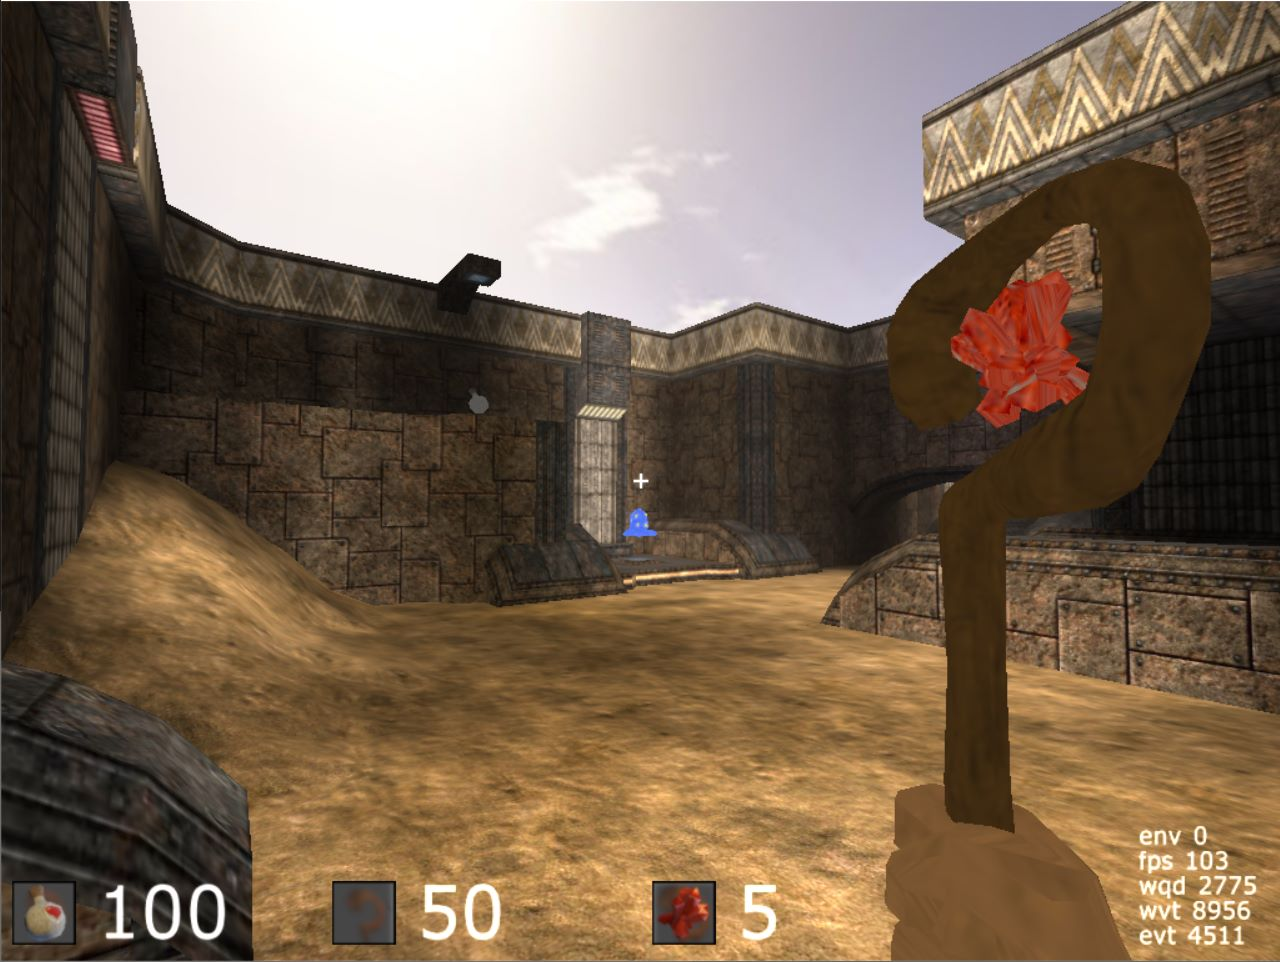
\includegraphics[width = 1\textwidth]{image10.jpg}
		\caption{A frame of the main character visual inside one scene of "Cube"}
	\end{center}
\end{figure}

\section{Middleware}
\begin{flushright}
	\itshape
	Why was middleware needed? Well, music and sound designers and programmers developed middleware \\
	so that the designers and composer could gain more control over how their audio was used in games.\\
	Middleware is based on the idea that the video game is an interactive medium, \\
	so all audio elements within the game should be interactive as well. \\
	\medskip
	--- Steve Horowitz and Scott Looney, "The essential guide to game audio "
\end{flushright}

Middlewares are softwares that sits between the game engine and the audio engine, providing a set of tools and features to manage audio content and processing. Middleware typically provides a layer of abstraction between the game engine and the audio engine.
Middleware can perform a variety of tasks, such as audio playback, dynamic mixing, audio processing, sound effects, and music management. It can also handle the integration of external audio tools and libraries, such as plug-ins. For example, Wwise can communicate with Steinberg Nuendo. In Wwise can be also loaded the plug-ins produced by Izotope for audio processing
When a game is being developed, the middleware receives audio data from the game engine, processes it according to the developer's settings, and sends the soundbanks to the audio engine for playback.
A Soundbank is a collection of audio files, that are packaged together into a single file for efficient loading and playback during the game.
Soundbanks typically contain metadata that describes how the audio files should be played back in the game, such as volume, panning, and spatial positioning information. Them are usually created using middleware tools and are loaded by the game engine during runtime. By using soundbanks, is possible to enabling a more immersive and dynamic audio experience in the game.
But why should i use a middleware? Without it, it will be more expensive in terms of time and energies, and the final result will not be the same as it would be with using the tools of a middleware, because the it's a computing enviroment developed to allow the sound designer to set the sound in a certain way, starting from the EQ up to the spatialization. You can do a lot of operations in a smart way that would otherwise require a lot of lines of code

\section{Wwise}
For my implementation i chose to use Wwise. But how does it work?
	
\begin{compactitem}
	\item Integration: Game developers integrate the Wwise Software Development Kit (SDK) into their game engine or application at the beginning of the project. Wwise usually comunicate with Unity and Unreal Engine. This allows the game engine to communicate with Wwise and utilize its audio features.
		
	\item Audio Asset Creation: Once the project has been created, the sound designers and the composers work on their music and sound with their own workflow on their favourite DAW (Digital audio workstation) and then load sounds into the Wwise hierarchy
		
	\item Project Setup: In Wwise, developers organize the imported audio assets into a project hierarchy.
		
	\item Sound Design and Mixing: Wwise provides a range of tools and features for sound design and mixing. Sound designers can define interactive behaviors and events, set up dynamic music systems, create spatial audio effects, and more.
		
	\item Integration with Game Events: Game events trigger specific audio actions within Wwise based on in-game events or conditions. For example, playing a gunshot sound effect when a player fires a weapon or triggering different music tracks based on the player's location or actions.
		
	\item Real-time Audio Processing: During gameplay, the game engine sends audio data requests to Wwise. Wwise processes these requests and provides the appropriate audio assets and information to the game engine, which then plays the audio in sync with the game's events and actions.
		
	\item Performance Optimization: Wwise offers various optimization features to ensure efficient and optimized audio processing. This includes streaming audio data, managing memory usage, and controlling resource usage based on gameplay priorities.
\end{compactitem}

\begin{figure}
	\begin{center}
		
\includegraphics[width=1\textwidth]{wwise.jpg}
		\caption{Wwise label}
	\end{center}
\end{figure}

To link a sound to a trigger, you need to create an event and put the sounds to play into it. The main section to work on to organize your work is the hierarchy. Here it is not only possible to order the types of events according to their purpose, but they can be grouped using functions that control certain playback parameters. 

	\subsection{Containers}
	Some of these events are grouped in differents containers. The containers are variations of the calling action of the differents events witch can trigger the sounds of the events in so many different ways. The containers that are mainly used are:
	
	\begin{compactitem}
		\item Simple Event: this is the simplest trigger container aviable in Wwise. This rappresent an audio event played once have been called.
		\item Random Container:  a set of audio events that are recalled randomly at each trigger. used for example for footsteps or jump sounds
		\item Switch Container: used to select severals audio events depending of a switch system.
		\item Blend Container: used to mix together different events, useful in the transitions. Used for example for different weapons, wich needs the trigger of the bullet drop and then his explotion.
		\item Sequence Container: reproduce the audio events contained in sequence, one after all, withoud interruption.
	\end{compactitem}

	\subsection{Dynamic controllers}
	Is also possible to control randomically some values through the game parameters.
	Game Parameters in Wwise are numeric variables that can be used to control audio behavior during application interaction. They are dynamic parameters that allow you to adjust different sound aspects in real time, such as volume, panning, transitions and more. Game Parameters offer a flexible way to create responsive and personalized audio interactions, also in randomic way. Is possible give to a game parameters a range of values in which to recall a parameter at each trigger, such as the volume, for example in a range from -12 and -3dB, or the cutoff frequency of a lowpass filter, for example from 200 to 1000 Hz.
	Some of these events are modulated by RTPC (Real-Time Parameter Control). It's a system that allows you to control the sound parameters in real time while playing the game.
	RTPC allows to change the values of a parameter, such as the volume, the pitch or the cutoff frequency of a filter, dynamically and based on events or situations that appeares in the game. For example, RTPC could be used to increase the volume of the sound when the player approaches a noise source, or to increase the pitch (so the playback speed) of the heartbeat sound based on the ammount of the healt of the character. In this way, a more immersive and realistic sound experience can be created for the player.
	
	\subsection{Actor-Mixer Hierarchy}
	To organize the events into the hierarchy of the project, use the Actor-Mixer
	In Wwise, an "Actor-Mixer" is a fundamental building block within the audio mixing hierarchy. It serves as a connection point for audio streams coming from different sounds or sound sources within a game. Actor-Mixers allow for effective grouping and control of sounds during the mixing phase.
	Within Wwise's mixing hierarchy, Actor-Mixers can contain other elements such as sounds, containers, States, and Switches. These elements represent specific sounds, containers, game states or control variables that can influence sound mixing, and switches that allow for selecting between different versions of a sound or effect.
	Actor-Mixers can also have routing connections to other Actor-Mixers or to the final output of the mixer, enabling the creation of a structured and flexible mixing hierarchy.
	By utilizing Actor-Mixers within Wwise, it becomes possible to efficiently organize and manage sounds within a project, facilitating control over the mixing and handling of audio levels within the context of an interactive application.
	
\section{Soundbanks of Cube}
The Wwise project of Cube is organized in 4 soundbanks wich contain all the events linked to the game triggers:
	
	\begin{compactitem}
		\item \textbf{Main} This soundbank contains the main sounds of player interaction through the game. It's also divided into 4 different Actor-Mixers:
			\begin{compactitem}
				\item Items: sounds linked to the events of the different scenes. The items are similar in each scene, but not at all: for example, the material of the floor changes, and consequently the sound of the player's footsteps or enemies also changes.
				I tried to denaturalize the footsteps sounds as much as possible, creating quick glitches or short clips sampled from high frequency sounding sources
				So each in this actor-mixer hierarchy are organized all the events of the scenes, such as the pick up gems sound, or the monster spawn sound.
				\item Magic: This section contains all the sound linked to the action of the weapon inside the game. The main character and the enemies have their own weapons, and consequently the weapon have their own sounds, wich are different for each weapon. This types of sounds are several, from the simple Staff Swing sound to more complex container, such as the FireGem Magic: this events contain 3 different sounds linked to different triggers: the Blast sound, the explode sound and the impact sound. This sound correspond to the different moments of use of some weapons, which involve actions of explosion of the shot from the gun, the impact of the shot with a surface and the explosion of the shot on the surface.
				For these sounds I used two types of sounds: hits followed by successions of high-frequency pulses, or sounds generated by additive synthesis, modulated by phasing, chorus or flanging which parameters are changed randomly at each trigger, so they never sound the same.
				\item Main Character: This actor-mixer hierarchy contain sounds linked to the physical action of the main character, like the voice sounds events, that is the sounds that the player makes when for example he is defeated or is hit by an enemy. This actor-mixer also contain the sound linked to other actions of the player such as jumping, breathing and impacting with some surfaces.
				For this type of event I decided to use short and nervous sounds, such as short successions of pulses or glitches, since these are sounds linked to triggers that comes with a high frequency, such as footstep triggers.
				I organized these sounds into random containers and randomized the control of some parameters like the pitch or the cutoff frequency of a LowPass Filter or a HighPass filter. So that, despite being repetitive events, they never sound the same.
				\item Monsters: These are the sounds linked to the physical actions of the enemies. This sounds are organized in 3 categories: Grunt, Pain and Defeated sounds.
				For these sounds I decided to use longer gestures, especially for the defeated sounds, because they are triggers that arrive after long intervals of time. I therefore took the opportunity to sample metallic sounds and modulate them with LFOs on different types of filters and AM and FM synthesis.
			\end{compactitem}
		
		\begin{figure}[h]
			\begin{center}
				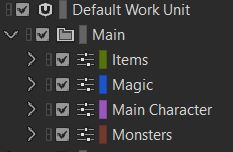
\includegraphics[width=.5\textwidth]{image1.jpg}
				\caption{Mixers-Hierarchy del soundbank \textbf{Main}}
			\end{center}
		\end{figure}
		
		\item \textbf{Music} Contains 3 events:
			\begin{compactitem}
				\item Blend Container wich contains 8 samples of flute notes, mixed together by the nature of the container. This event is linked to the trigger of the appearance of the main enemy
				\item Arpeggio Synth
				\item Melody Synth
			\end{compactitem}
		\begin{figure}[h]
			\begin{center}
				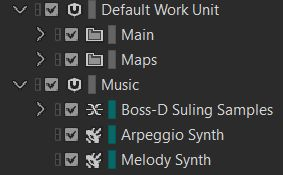
\includegraphics[width=.5\textwidth]{image2.jpg}
				\caption{Mixers-Hierarchy del soundbank \textbf{Music}}
			\end{center}
		\end{figure}
		
		\item \textbf{DCP-the-core} Contains all initialization sounds: game start sounds and various initial sound of the scenes (maps). This soundbank contains the main background track called "Cubetrack", which lasts 04:40 and is played in loop during the game session.
		\item \textbf{Init} This is the auto-defined soundbank. Thys type of soundbank is automatically generated by the Wwise audio authoring tool based on the project's content and settings.		
		With auto-defined soundbanks, Wwise automatically determines which audio assets should be included in each soundbank based on their usage and dependencies within the project.
	\end{compactitem}

	\begin{figure}[h]
		\begin{center}
			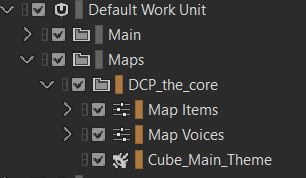
\includegraphics[width=.5\textwidth]{image3.jpg}
			\caption{Mixers-Hierarchy del soundbank \textbf{DCP-the-core}}
		\end{center}
	\end{figure}

\section{Electroacoustic gestures}
As mentioned before, each musical gesture through the implementation has his own role in the electroacoustic compositional view.

	\subsection{Aesthetics}
	Now let's explore how I assigned several musical gestures to specific actions, and how they create an environment when they are added together. There are 3 basic ideas from which I move to make these decisions
		\begin{enumerate}
			\item Assign short nervous and never repetitive gestures to frequently repeated actions
			\item Assign long and dilated gestures to actions that are repeated infrequently in the game
			\item Try to predict the probabilities with which some sounds will be recalled together and therefore overlap. based on this I try to give musical roles to each of them. I organize the implementation in such a way that 3 types of sounds are never missing during the game
				\begin{compactitem}
					\item Percussive and pulsation sounds that give movement to gestures
					\item Low frequency sounds to support the
					\item Quick and dynamic hig frequency gestures
				\end{compactitem}
		\end{enumerate}
	
	\subsection{EQ}
	I organized the equalization of the material according to the criteria mentioned above, even if it is statistically very difficoult to be able in predicting which sounds will play together and how, mainly for two reasons:
	
	\begin{compactitem}
		\item as already mentioned, a video game have non-linear events, and consequently unpredictable events
		\item as already mentioned, many sound parameters are modified randomly with each trigger, consequently the possibilities of creating different timbres increase
	\end{compactitem}
	
	So I tried to equalize the sounds in an optimal way trying to obtain a balanced result in the spectrum, limiting the variations of some parameters such as time stretching and reverb so that they do not change the timbre too much. Consequently I have tried to make coherent choices, trying to maintain a distinction between percussive and non-percussive sounds, between background and melodic sounds.

\begin{comment}
\begin{code}
\documentclass[\meta{\dots\unkern}]{scrreprt} % or scrbook or scrartcl

\usepackage[\meta{\dots\unkern}]{classicthesis}
\usepackage{arsclassica}

\begin{document}
\dots
\end{document}
\end{code}

For example, this document has been produced with the following code:
\begin{code}
\documentclass[a4paper,twoside,openright,titlepage,
               headinclude,footinclude,BCOR5mm,
               numbers=noenddot,cleardoublepage=empty,
               tablecaptionabove]{scrreprt}

\usepackage{\meta{\dots\unkern}}
\usepackage{subfig}
\usepackage[eulerchapternumbers,subfig,beramono,eulermath,pdfspacing]%
           {classicthesis}
\usepackage{arsclassica}

\begin{document}
\dots
\end{document}
\end{code}

It is recommended to use the \optname{beramono} and \optname{eulerchapternumbers} options together with \arsclassica.



\section{Style}

The typographical style achieved with \arsclassica{} differs from \classicthesis{} in the following points:
\begin{itemize}
\item use of Iwona font, by Janusz Nowacki, for the sectioning unit titles (chapters, sections, subsections, sub-subsections, paragraphs and subparagraphs), for the description list labels, the headlines and the caption labels (\classicthesis{} doesn't use any sans serif font);
\item customized chapter numbers;
\item semi-transparent headlines; the headlines are separated from the page number by a small rule;
\item caption labels in boldface (\classicthesis{} doesn't use any boldface font);
\item itemize lists with semi-transparent bullets.
\end{itemize}

\arsclassica{} is designed  to provide a ready-to-use typographical style: for this reason it has no loading options and it is \emph{not} configurable or customizable in any way. If you change the previous settings, you'll risk to destroy the balance of the style, so it is \emph{highly recommended} to keep them unchanged.

One of the principles of \LaTeX{} is that it allows the author to take no interest in the typographical questions, permitting him to focus only on the structure and the contents of his document. This fact should always be kept in mind: using a style written by others, the user accepts all the typographical settings chosen for him by the author of the style, and he isn't forced to study typography to fine-tune the layout of his publications. This is the case of \arsclassica{} too: if you change its settings, you'll deny this philosophy and, consequently, you'll have to study (a lot of) typography to achieve acceptable results.

The style achieved with \arsclassica{} is \emph{not} therefore configurable or customizable. The typographical style is very personal: if you like this package and find attractive the idea to take no interest in the problem of the style definition, then you'll use \arsclassica{} with satisfaction; otherwise, if you have different needs or you aren't satisfied with the layout of the package, then you should try other classes or packages, even building your own style.



\section{Important}

To write a document according to the \arsclassica{} style, you have to follow some very simple rules.
\begin{itemize}
\item Don't change \emph{for any reason} the \arsclassica{} settings (fonts, text body size, colors, \dots).
\item The sectioning unit titles (chapters, section, subsections, \dots) have to be \emph{one line long}, possibly in \emph{plain text} (no symbols, formulas or code fragments). If you have titles longer than one line, try and rephrase them: you can almost always do it.
\item In the table of contents and in the list of tables and figures, captions have to be \emph{one line long}, possibly in \emph{plain text}. Use the optional argument of sectioning commands and of \cmdname{caption}, if necessary.
\item Don't use \optname{tocaligned} and \optname{dottedtoc} options of \classicthesis: the default table of contents does the job very well (see the documentation of \classicthesis{} for a nice discussion of this point).
\item Don't use vertical or double rules in your tables (see the documentation of \pkgname{booktabs}).
\item Use footnotes and margin notes very sparingly.
\item If your document includes graphs and plots, draw them using \LaTeX{} (by \pkgname{Ti\emph{k}Z} and \pkgname{pgfplots}, for example) and not an external software. This is the only way to get the best typographical outcome.
\end{itemize}



\section{Examples}

%\begin{figure}
%\centering
%\subfloat[Asia personas duo]
%{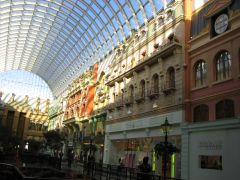
\includegraphics[width=.45\columnwidth]{Lorem}} \quad
%\subfloat[Pan ma signo]
%{\label{fig:example-b}%
%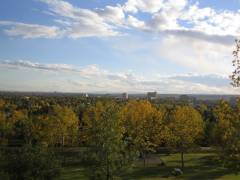
\includegraphics[width=.45\columnwidth]{Ipsum}} \\
%\subfloat[Methodicamente o uno]
%{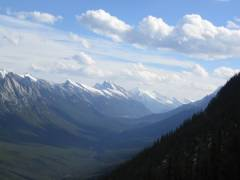
\includegraphics[width=.45\columnwidth]{Dolor}} \quad
%\subfloat[Titulo debitas]
%{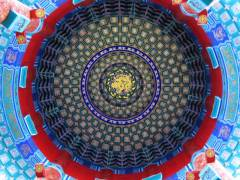
\includegraphics[width=.45\columnwidth]{Sit}}
%\caption[Tu duo titulo debitas latente]{Tu duo titulo debitas latente}
%\label{fig:example}
%\end{figure}

Please note that the content of this section is just some dummy text. It isn't a real language.

Lorem ipsum dolor sit amet, consectetuer adipiscing elit. Ut purus elit, vestibulum ut, placerat ac, adipiscing vitae, felis. Curabitur dictum gravida mauris.

\subsection*{A subsection}

\lipsum[2]

\subsubsection*{A sub-subsection}

\lipsum[7]

\paragraph{A paragraph}
Lorem ipsum dolor sit amet, consectetuer adipiscing elit. Ut purus elit, vestibulum ut, placerat ac, adipiscing vitae, felis. Curabitur dictum gravida mauris. Nam arcu libero, nonummy eget, consectetuer id, vulputate a, magna.

\paragraph{Another paragraph}
Cras nec ante, pellentesque a nulla, cum sociis natoque penatibus et magnis dis parturient montes, nascetur ridiculus mus. Aliquam tincidunt urna

\bigskip

Donec aliquet, tortor sed accumsan bibendum, erat ligula aliquet magna, vitae ornare odio metus a mi. Morbi ac orci et nisl hendrerit mollis. Suspendisse ut massa. Cras nec ante. Pellentesque a nulla. Cum sociis natoque penatibus et magnis dis parturient montes, nascetur ridiculus mus. Aliquam tincidunt urna.

\begin{description}
\item[Mane] Lorem ipsum dolor sit amet, consectetuer adipiscing elit.
\item[Tekel] Ut purus elit, vestibulum ut, placerat ac, adipiscing vitae, felis. Curabitur dictum gravida mauris.
\item[Fares] Nam arcu libero, nonummy eget, consectetuer
id, vulputate a, magna.
\end{description}

\begin{table}
\caption{Lorem ipsum dolor sit amet}
\centering
\begin{tabular}{ll}
\toprule
\textbf{Alkaloid} & \textbf{Origin} \\
\midrule
atropine & belladonna \\
morphine & poppy \\
nicotine & tobacco \\
\bottomrule
\end{tabular}
\end{table}

Suspendisse vel felis. Ut lorem lorem, interdum eu, tincidunt sit amet, laoreet vitae, arcu. Aenean faucibus pede eu ante. Praesent enim elit, rutrum at, molestie non, nonummy vel, nisl. Ut lectus eros, malesuada sit amet, fermentum eu, sodales cursus, magna. Donec eu purus. Quisque vehicula, urna sed ultricies auctor, pede lorem egestas dui, et convallis elit erat sed nulla.

\subsection*{Some formulas}

Una formula in linea viene incorporata nel testo: $\lim_{n \to \infty}\sum_{k=1}^n \frac{1}{k^2} = \frac{\pi^2}{6}$, per esempio. Come si osserva, \LaTeX{} fa \emph{il possibile} per comprimerla e modificare il meno possibile l'interlinea nel capoverso che la contiene.
Una formula in display viene invece composta da \LaTeX{} su linee a parte, separate dal contesto con adeguati spazi bianchi per metterla in mostra e farla risaltare sulla pagina.
\begin{equation}
\lim_{n \to \infty}\sum_{k=1}^n \frac{1}{k^2}= \frac{\pi^2}{6}
\end{equation}
Come si osserva, ora la formula risulta centrata, non compressa, e tutti i suoi elementi occupano il giusto spazio con un risultato finale di grande respiro.

Integer tempus convallis augue. Etiam facilisis. Nunc elementum fermentum wisi. Aenean placerat. Ut imperdiet, enim sed gravida sollicitudin, felis odio placerat quam, ac pulvinar elit purus eget enim.

\begin{equation}
\int_a^{a+T}f(x)\,dx= \int_0^T f(x)\,dx
\qquad
\oint f(z)\,dz=2\pi i
\end{equation}

Nulla malesuada porttitor diam. Donec felis erat, congue non, volutpat at, tincidunt tristique, libero. Vivamus viverra fermentum felis. Donec non- ummy pellentesque ante.

\begin{equation}
f(x_1,\dots,x_n)=  \prod_{k=1}^n x_k
\qquad
\sum_{k=1}^n x_k^2=1
\qquad
\biggl(\sum_n x_n^2\biggr)^{1/2}
\end{equation}

\lipsum[2]

\begin{equation}
\begin{bmatrix}
a_{11} & \dots & a_{1n} \\
a_{21} & \dots & a_{2n} \\
\hdotsfor{3} \\
a_{n1} & \dots & a_{nn}
\end{bmatrix}
\end{equation}

\lipsum[4]

\begin{equation}
\lim_{x\to 0}
\frac{\sin x}{x}=1 \qquad
\lim_{n\to +\infty}f_n=\delta
\end{equation}

Fusce mauris. Vestibulum luctus nibh at lectus. Sed bibendum, nulla a faucibus semper, leo velit ultricies tellus, ac venenatis arcu wisi vel nisl. Vestibulum diam.

\begin{equation}
n!=
\begin{cases}
1       & \text{if $n=0$} \\
n(n-1)! & \text{if $n\ge 1$}
\end{cases}
\end{equation}

Ut lectus eros, malesuada sit amet, fermentum eu, sodales cursus, magna. Donec eu purus. Quisque vehicula, urna sed ultricies auctor, pede lorem egestas dui, et convallis elit erat sed nulla. Donec luctus. Curabitur et nunc. Aliquam dolor odio, commodo pretium, ultricies non, pharetra in, velit.

\begin{equation}
x_G=
\frac{\displaystyle
      \sum_{i=1}^n m_ix_i}
{\displaystyle\sum_{i=1}^n m_i}
\end{equation}

\lipsum[6]

\begin{equation}
\kappa =\frac{\xi}{E_{\textrm{max}}}
\qquad
E_{\textup{max}} =\frac{2 m_{\textup{e}} \beta^2\gamma^2 }{1 +2\gamma m_{\textup{e}}/m_{\textrm{x}} + ( m_{\textup{e}}/m_{\textup{x}})^2}
\end{equation}

\lipsum[8]
\end{comment}